\begin{pastexam}[label={px:nchu-114-dsa-25}]{中興資工所甲組 114 學年度 計算題第 5 題}
（計算）

Consider a binary min-heap represented by the array \textbf{[1, 3, 2, 10, 7, 6, 9]}, where the element 1 is at the root. Suppose you need to insert a new element, 4, into this min-heap. Describe the complete insertion process step-by-step. Your answer should include (10 \%):
\begin{itemize}
\item Indicating where the new element is initially placed in the array.
\item Explaining the heapify-up (or bubble-up) process in detail, showing each intermediate state of the heap after any necessary swaps.
\item Presenting the final min-heap array once the insertion is complete.
\end{itemize}
Make sure to clearly justify the steps taken and the reasoning behind each comparison and swap, based on the fundamental properties of a min-heap.
\end{pastexam}

\begin{pastsoln}
答案：最後的陣列是 $[1, 3, 2, 4, 7, 6, 9, 10]$。

\textbf{約定}。 陣列從 $1$ 開始編號：$A[i]$ 的父節點是 $A[\lfloor i/2 \rfloor]$，子節點是 $A[2i]$、$A[2i+1]$
（資結書第~8.1~節）。 最小堆積有兩個性質：形狀是完全二元樹（陣列中間沒有空格）；每個節點都 $\le$ 它的
子節點，所以根是最小值。 原本的堆積：
\begin{center}
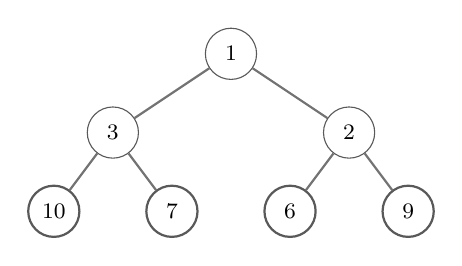
\begin{tikzpicture}[level distance=10mm, edge from parent/.style={draw=black!55, thick},
  every node/.style={circle, draw=black!65, minimum size=6.5mm, inner sep=0pt, font=\footnotesize},
  level 1/.style={sibling distance=30mm}, level 2/.style={sibling distance=15mm}]
\node {1}
  child {node {3} child {node {10}} child {node {7}}}
  child {node {2} child {node {6}} child {node {9}}};
\end{tikzpicture}
\end{center}
檢查一下它確實是最小堆積：$1 \le 3, 2$；$3 \le 10, 7$；$2 \le 6, 9$。

\textbf{第一步：放在陣列最後}。 為了維持完全二元樹的形狀，新元素只能放在下一個空位，也就是 $A[8]$
（最後一層最左邊的空位，$A[4] = 10$ 的左子節點）。 陣列變成 $[1, 3, 2, 10, 7, 6, 9, \mathbf{4}]$。 這時形狀
正確，但 $4$ 和它的父節點可能違反大小關係，要往上調（資結書虛擬碼~8.2 的 \proc{Heap-Insert}，最小堆積
把比較反過來）。

\textbf{第二步：往上浮}。 每一步比較新元素和它的父節點，父節點比較大就交換。
\begin{center}
\begin{tabular}{clll}
\toprule
新元素位置 $i$ & 父節點 $A[\lfloor i/2 \rfloor]$ & 比較 & 動作與交換後的陣列 \\
\midrule
$8$ & $A[4] = 10$ & $4 < 10$ & 交換：$[1, 3, 2, \mathbf{4}, 7, 6, 9, 10]$ \\
$4$ & $A[2] = 3$ & $4 \ge 3$ & 停止 \\
\bottomrule
\end{tabular}
\end{center}
第一次比較：$4$ 的父節點 $10$ 比它大，違反「父 $\le$ 子」，交換後 $4$ 到了 $A[4]$，$10$ 下到 $A[8]$。 這時
$4$ 唯一的子節點是 $10$，$4 \le 10$ 成立；其他位置沒有變動。 第二次比較：$4$ 的父節點 $A[2] = 3 \le 4$，大小關係
成立；再往上的祖先 $1$ 本來就 $\le 3$，所以整棵樹都滿足堆積性質，停止。

\textbf{最後的堆積}：$[1, 3, 2, 4, 7, 6, 9, 10]$。
\begin{center}
\begin{tikzpicture}[level distance=10mm, edge from parent/.style={draw=black!55, thick},
  every node/.style={circle, draw=black!65, minimum size=6.5mm, inner sep=0pt, font=\footnotesize},
  level 1/.style={sibling distance=30mm}, level 2/.style={sibling distance=15mm}, level 3/.style={sibling distance=8mm}]
\node {1}
  child {node {3} child {node[draw=optStroke, thick, fill=optFill] {4} child {node {10}} child[missing]} child {node {7}}}
  child {node {2} child {node {6}} child {node {9}}};
\end{tikzpicture}
\end{center}
逐一檢查：$1 \le 3, 2$；$3 \le 4, 7$；$2 \le 6, 9$；$4 \le 10$。 一共比較 $2$ 次、交換 $1$ 次。 一般而言，往上浮最多
走到根，次數不超過樹高 $\lfloor \lg n \rfloor$，插入是 $O(\log n)$。
\end{pastsoln}
